
% - Description du capteur
% 		- Le matériel
% 		- Le système d'exploitation Zephyr
% 		- La couche radio LoRa
%      - Le logiciel embarqué
%		- Le boîtier

\chapter{Description du capteur}\label{ch:capteur}

Le travail du capteur et d'acquérir les données nécessaires, puis de les transmettre à intervalles réguliers par la couche radio LoRa aux passerelles. Le cœur du capteur est le micro-contrôleur, celui-ci permet l'exécution du firmware qui est en charge de la gestion des opérations. C'est cette application qui va effectuer aux moments voulus les acquisitions nécessaire et ensuite créer un paquet de données pour être  envoyé.

Pour se faire le capteur est munit de plusieurs modules permettant l'acquisition des différents paramètres. Il sont présentés dans la liste suivante.

\begin{itemize}
\item GPS: Il permettra de connaître la position (latitude/longitude) du capteur
\item Accéléromètre: Ce module sera utilisé pour connaître le nombre de pas effectué par le sportif ce qui permettra de calculer sa cadence
\item Rythme cardiaque:  Au moyen d'une sangle pectorale portée par l'athlète, ce module déclenchera une impulsion à chaque fois qu'un battement du cœur sera détecté
\item Radio LoRa: C'est au moyen de cet élément que le capteur transmettra les paquets de données
\end{itemize}

\section{Le matériel}

Lors de la pré-étude du projet, trois différentes cartes avaient été étudiée chacune avec leurs avantages et inconvénients. Pour la réalisation du projet, j'ai décidé d'utiliser la carte qui dispose de base du plus de module, c'est à dire la SODAQ One. En effet elle a l'immense avantage d'embarquer de base un module LoRa, un module GPS ainsi qu'un accéléromètre ce qui me permet de me focaliser sur le développement du logiciel embarqué. Il reste seulement à connecter sur une entrée du micro-contrôleur le module qui permettra de compter les battements du cœur en détectant les impulsions produite. Enfin afin de faciliter le debug de l'application embarquée, un UART sera également connecté pendant la phase de debug ce qui permettra d'afficher des messages.

Pour rappel, les caractéristiques du SODAQ One sont décrit dans la table~\ref{tab:sodaq_one_cara}.

\begin{table}[htb]
\caption[Caractéristiques de la carte SODAQ One v3]{Caractéristiques de la carte SODAQ One v3}
\label{tab:sodaq_one_cara}
\centering
\begin{tabular}{ l | l }
\toprule
Dimensions & 45mm x 25mm \\
\midrule
Microcontrôleur & ATSAMD21G18 – ARM Cortex M0 \\
\midrule
Oscillateur & 48 Mhz \\
\midrule
Flash & 256 kB \\
\midrule
RAM & 32 kB \\
\midrule
LoRa & Microchip RN2483 \\
\midrule
GPS & uBlox EVA 8M \\
\midrule
Accéléromètre & STMicroelectronics LSM303AGR \\
\midrule
Prix & 114 CHF\\
\bottomrule 
\end{tabular}
\end{table}

Aux modules de base, comme expliqué précédemment, il faudra rajouter un module qui permettra de compter le nombre de battement du cœur. Il est développé par la société Adafruit sous le nom de "Adafruit Heart Rate Start Pack".

\hl{PHOTO SODAQ}

Le module LoRa RN2483 est connecté par un lien série UART et utilise une interface de type AT commands, c'est à dire qu'il est piloté avec l'envoie de chaînes de caractère représentant des commandes, dans la même idée les réponses reçues sont de type text. Le module GPS ainsi que l'accéléromètre sont quant à eux connecté sur le bus $I^{2}C$. Le module rythme cardiaque sera lui connecté simplement sur un General Purpose I/O.

% Configuration HW? i.e. nb msg GPS etc..

Le schéma block~\ref{fig:schema_block_sodaq} présente les différents modules et leurs connections avec le micro-contrôleur.

\begin{figure}[htb]
\centering 
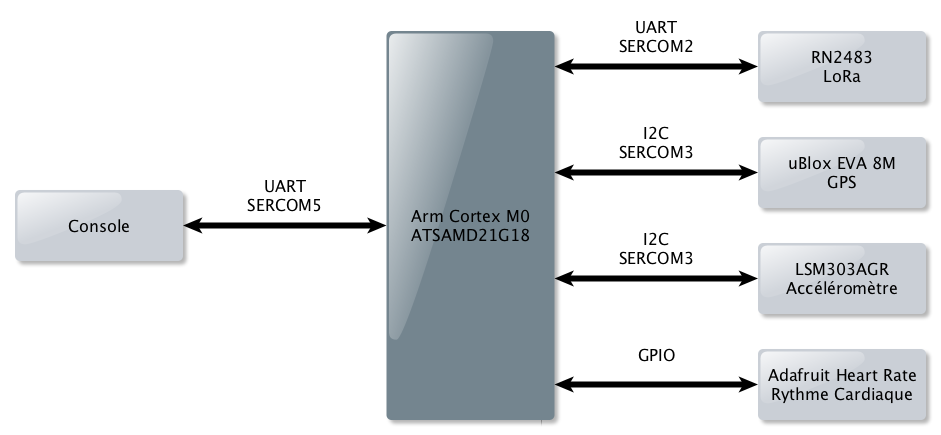
\includegraphics[width=1\columnwidth]{sensor_schema} 
\caption{Schéma block du capteur SODAQ One}
\label{fig:schema_block_sodaq}
\end{figure}

\section{Le système d'exploitation Zephyr}

\hl{TODO}

\section{Le logiciel embarqué}

\hl{TODO}

\section{Le boîtier}

\hl{TODO}
